
\documentclass[11pt,letterpaper]{article}
\usepackage[top=0.85in,left=2.75in,footskip=0.75in]{geometry}


\usepackage{amsmath,amssymb}


\usepackage{changepage}


\usepackage[utf8x]{inputenc}


\usepackage{textcomp,marvosym}


\usepackage{cite}


\usepackage{nameref,hyperref}


\usepackage[right]{lineno}


\usepackage{microtype}
\DisableLigatures[f]{encoding = *, family = * }


\usepackage[table]{xcolor}


\usepackage{array}


\newcolumntype{+}{!{\vrule width 2pt}}


\newlength\savedwidth
\newcommand\thickcline[1]{
  \noalign{\global\savedwidth\arrayrulewidth\global\arrayrulewidth 2pt}
  \cline{#1}
  \noalign{\vskip\arrayrulewidth}
  \noalign{\global\arrayrulewidth\savedwidth}
}


\newcommand\thickhline{\noalign{\global\savedwidth\arrayrulewidth\global\arrayrulewidth 2pt}%
\hline
\noalign{\global\arrayrulewidth\savedwidth}}


\raggedright
\setlength{\parindent}{0.5cm}
\textwidth 5.25in 
\textheight 8.75in


\usepackage[aboveskip=1pt,labelfont=bf,labelsep=period,justification=raggedright,singlelinecheck=off]{caption}
\renewcommand{\figurename}{Fig}

\makeatletter
\renewcommand{\@biblabel}[1]{\quad#1.}
\makeatother




\usepackage{lastpage,fancyhdr,graphicx}
\graphicspath{ {./paperImages/} }
\usepackage{epstopdf}

\pagestyle{fancy}
\fancyhf{}

\rfoot{\thepage}
\renewcommand{\headrulewidth}{0pt}
\renewcommand{\footrule}{\hrule height 2pt \vspace{2mm}}
\fancyheadoffset[L]{2.25in}
\fancyfootoffset[L]{2.25in}
\lfoot{\today}

\begin{document}
\vspace*{0.2in}

\begin{flushleft}
{\Large
\textbf\newline{Non-Local Means Denoising}
}
\newline

\\
fdmw97
\\
\bigskip

\end{flushleft}

\section*{Algorithm Description}
The Non-Local Means algorithm takes an image $v$ consiting of $I$ pixels. Then for each pixel $i \in I$ produces a new value for $i$ that is the result of a a weighted average of all the pixels in the image. This is described by the formula
$$\mathit{NL}[\mathit{u](x)} = \frac{1}{\mathit{C(x)}}\int_{\Omega}^{}\mathit{e^{-\frac{(G_{a}*|u(x+.)-u(y+.)|^{2})(0)}{h^{2}}u(y) dy}}$$
where $\mathit{x \in \Omega, C(x) = \int_{\Omega}^{}e^{-\frac{(G_{a}*|u(x+.)-u(z+.)|^{2})(0)}{h^{2}}dz}}$ is a normalizing constant\cite{paper1}
In this formula $h$ serves as an adjustable parameter to change the filtering of the image. From the above formula it can be seen that this algorithm weights the pixels in the image such that a pixel is only modified by pixels situated in gaussian neighbourhoods similar to that of $x$.
For the algorithm to be sensibly implemented the above formula must be reformulated into a discrete algorithm. Examples of these are discussed below.

\section*{Algorithm Implementations}
\paragraph{Pixelwise Implementation:}
The first discrete implementation I will be discussing is the Pixelwise Implementation. This implementation is the most faithful to the original formula given for the algorithm since it calculates the denoised value for a pixel $p$ one pixel at a time. The algorithm proposed in \cite{paper2} is as follows.
$u = (u_{1}, u_{2}, u_{3})$ is a colour image, if a pixel $p$ is selected its new value is given by
$$\mathit{\hat{u_{i}}(p) = \frac{1}{C(p)} \sum_{q\in B(p,r)}^{}u_{i}(q)w(p,q)}\text{,    }\mathit{C(p)=\sum_{q\in B(p,r)}^{}w(p,q)},$$
where $i$ = 1, 2, 3 and $B(q,r)$ is a neighbourhood centered on pixel $p$ with size $\mathit{(2r+1)\times (2r+1)}$. $r$ is used to restrict the neighbourhood size depending on the standard deviation of the noise in the image so that the algorithm performs in a reasonable amount of time. $w(p,1)$ is the weight for the average and is dependant on the squared Euclidean distance between 2 neighbourhoods $B(p,f)$ and $B(q,f)$ the result is given by 
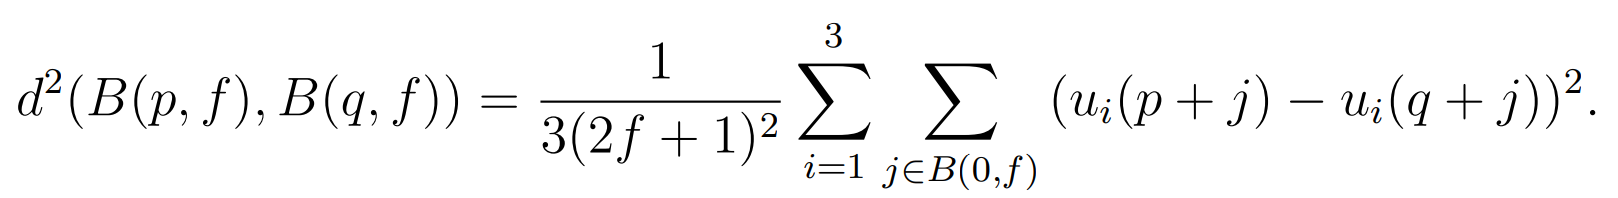
\includegraphics{weighted}
the weight $w(p,q)$ is then given by the formula
\begin{figure}
\centering
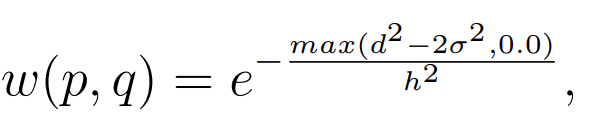
\includegraphics{w}
\end{figure}
$h$ is the filtering parameter discussed in \cite{paper1} This formula gives higher weightings to more similar patches. Setting patches with a distance less than twice the variance of the noise to 1 and all other patches to rapidly decreasing values less than 1. $p$ is set to the largest of the weights in $B(P,r)$ so that it is not unfairly weighted in the average. Every pixel in $u$ is passed into this algorithm and the resulting pixels form the denoised image.
\paragraph{Patchwise Implementation}

\begin{thebibliography}{9}
\bibitem{paper1}
Antoni Buades, and Jean-Michel Morel.
\textit{A non-local algorithm for image denoising}.
In Proceedings of the 2005 IEEE Computer Society Conference on Computer Vision and Pattern Recognition (CVPR’05) - Volume 2 - Volume 02 (CVPR ’05). IEEE Computer Society, USA, 60–65.

\bibitem{paper2}
Antoni Buades, Bartomeu Coll, and Jean-Michel Morel
\textit{Non-Local Means Denoising}.
Image Processing Online.


\end{thebibliography}



\end{document}

